%File: formatting-instructions-latex-2024.tex
%release 2024.0
\documentclass[letterpaper]{article} % DO NOT CHANGE THIS
\usepackage{aaai24}  % DO NOT CHANGE THIS
\usepackage{times}  % DO NOT CHANGE THIS
\usepackage{helvet}  % DO NOT CHANGE THIS
\usepackage{courier}  % DO NOT CHANGE THIS
\usepackage[hyphens]{url}  % DO NOT CHANGE THIS
\usepackage{graphicx} % DO NOT CHANGE THIS
\urlstyle{rm} % DO NOT CHANGE THIS
\def\UrlFont{\rm}  % DO NOT CHANGE THIS
\usepackage{natbib}  % DO NOT CHANGE THIS AND DO NOT ADD ANY OPTIONS TO IT
\usepackage{caption} % DO NOT CHANGE THIS AND DO NOT ADD ANY OPTIONS TO IT
\frenchspacing  % DO NOT CHANGE THIS
\setlength{\pdfpagewidth}{8.5in}  % DO NOT CHANGE THIS
\setlength{\pdfpageheight}{11in}  % DO NOT CHANGE THIS
%
% These are recommended to typeset algorithms but not required. See the subsubsection on algorithms. Remove them if you don't have algorithms in your paper.
\usepackage{algorithm}
\usepackage{algorithmic}
\usepackage{booktabs}


%
% These are are recommended to typeset listings but not required. See the subsubsection on listing. Remove this block if you don't have listings in your paper.
\usepackage{newfloat}
\usepackage{listings}
\DeclareCaptionStyle{ruled}{labelfont=normalfont,labelsep=colon,strut=off} % DO NOT CHANGE THIS
\lstset{%
	basicstyle={\footnotesize\ttfamily},% footnotesize acceptable for monospace
	numbers=left,numberstyle=\footnotesize,xleftmargin=2em,% show line numbers, remove this entire line if you don't want the numbers.
	aboveskip=0pt,belowskip=0pt,%
	showstringspaces=false,tabsize=2,breaklines=true}
\floatstyle{ruled}
\newfloat{listing}{tb}{lst}{}
\floatname{listing}{Listing}
%
% Keep the \pdfinfo as shown here. There's no need
% for you to add the /Title and /Author tags.
\pdfinfo{
/TemplateVersion (2024.1)
}

% DISALLOWED PACKAGES
% \usepackage{authblk} -- This package is specifically forbidden
% \usepackage{balance} -- This package is specifically forbidden
% \usepackage{color (if used in text)
% \usepackage{CJK} -- This package is specifically forbidden
% \usepackage{float} -- This package is specifically forbidden
% \usepackage{flushend} -- This package is specifically forbidden
% \usepackage{fontenc} -- This package is specifically forbidden
% \usepackage{fullpage} -- This package is specifically forbidden
% \usepackage{geometry} -- This package is specifically forbidden
% \usepackage{grffile} -- This package is specifically forbidden
% \usepackage{hyperref} -- This package is specifically forbidden
% \usepackage{navigator} -- This package is specifically forbidden
% (or any other package that embeds links such as navigator or hyperref)
% \indentfirst} -- This package is specifically forbidden
% \layout} -- This package is specifically forbidden
% \multicol} -- This package is specifically forbidden
% \nameref} -- This package is specifically forbidden
% \usepackage{savetrees} -- This package is specifically forbidden
% \usepackage{setspace} -- This package is specifically forbidden
% \usepackage{stfloats} -- This package is specifically forbidden
% \usepackage{tabu} -- This package is specifically forbidden
% \usepackage{titlesec} -- This package is specifically forbidden
% \usepackage{tocbibind} -- This package is specifically forbidden
% \usepackage{ulem} -- This package is specifically forbidden
% \usepackage{wrapfig} -- This package is specifically forbidden
% DISALLOWED COMMANDS
% \nocopyright -- Your paper will not be published if you use this command
% \addtolength -- This command may not be used
% \balance -- This command may not be used
% \baselinestretch -- Your paper will not be published if you use this command
% \clearpage -- No page breaks of any kind may be used for the final version of your paper
% \columnsep -- This command may not be used
% \newpage -- No page breaks of any kind may be used for the final version of your paper
% \pagebreak -- No page breaks of any kind may be used for the final version of your paperr
% \pagestyle -- This command may not be used
% \tiny -- This is not an acceptable font size.
% \vspace{- -- No negative value may be used in proximity of a caption, figure, table, section, subsection, subsubsection, or reference
% \vskip{- -- No negative value may be used to alter spacing above or below a caption, figure, table, section, subsection, subsubsection, or reference

\setcounter{secnumdepth}{0} %May be changed to 1 or 2 if section numbers are desired.

% The file aaai24.sty is the style file for AAAI Press
% proceedings, working notes, and technical reports.
%

% Title

% Your title must be in mixed case, not sentence case.
% That means all verbs (including short verbs like be, is, using,and go),
% nouns, adverbs, adjectives should be capitalized, including both words in hyphenated terms, while
% articles, conjunctions, and prepositions are lower case unless they
% directly follow a colon or long dash
\title{A Quantum-Classical Machine Learning Comparison for Malware Detection}
\author{
    %Authors
    % All authors must be in the same font size and format.
    Mary L. Cotrupi\textsuperscript{\rm 1}, Allison Aurilio\textsuperscript{\rm 2}, Sean Sanpietro\textsuperscript{\rm 3}, Fabiana Torres\textsuperscript{\rm 4}, Anwita Kasturi\textsuperscript{\rm 1}, Quinn Colognato\textsuperscript{\rm 1}, Brian Robert Callahan\textsuperscript{\rm 4}
}
\affiliations{
    %Afiliations
    \textsuperscript{\rm 1}Dept. of Computer Science, Rensselaer Polytechnic Institute, Troy, NY 12180-3590 USA\\
    \textsuperscript{\rm 2}Dept. of Electrical and Computer Engineering, The College of New Jersey, 2000 Pennington Road, Ewing, NJ 08618-1100 USA\\
    \textsuperscript{\rm 3}Dept. of Computer Science, Misericordia University, 301 Lake Street, Dallas, PA 18612-7752 USA\\
    \textsuperscript{\rm 4}Dept. of Computer Science and Software Engineering, Monmouth University, 400 Cedar Avenue, West Long Branch, NJ 07764-1828 USA\\
    cotrum@rpi.edu, aurilia2@tcnj.edu, ssanpiet@misercordia.edu, s1378769@monmouth.edu, kastua@rpi.edu, cologq@rpi.edu, bcallaha@monmouth.edu
}

%Example, Single Author, ->> remove \iffalse,\fi and place them surrounding AAAI title to use it
\iffalse
\title{My Publication Title --- Single Author}
\author {
    Author Name
}
\affiliations{
    Affiliation\\
    Affiliation Line 2\\
    name@example.com
}
\fi

\iffalse
%Example, Multiple Authors, ->> remove \iffalse,\fi and place them surrounding AAAI title to use it
\title{My Publication Title --- Multiple Authors}
\author {
    % Authors
    First Author Name\textsuperscript{\rm 1,\rm 2},
    Second Author Name\textsuperscript{\rm 2},
    Third Author Name\textsuperscript{\rm 1}
}
\affiliations {
    % Affiliations
    \textsuperscript{\rm 1}Affiliation 1\\
    \textsuperscript{\rm 2}Affiliation 2\\
    firstAuthor@affiliation1.com, secondAuthor@affilation2.com, thirdAuthor@affiliation1.com
}
\fi


% REMOVE THIS: bibentry
% This is only needed to show inline citations in the guidelines document. You should not need it and can safely delete it.
\usepackage{bibentry}
% END REMOVE bibentry

\begin{document}

\maketitle

\begin{abstract}
Quantum Machine Learning (QML) is beginning to show potential promise as an emerging technology for a myriad of cybersecurity tasks. One such task is malware detection, which remains a difficult and critical problem both for individuals and today's organizations. While there is a growing literature on applying QML to malware analysis, many remained confined only to simulators, leaving open the question of how do theoretical simulation insights apply to real-world Noisy Intermediate-Scale Quantum (NISQ) machines that exist today. In this paper, we provide a four-way comparison of four malware datasets between classical machine learning, QML performed on the Qiskit Aer simulator without noise and with noise, and QML performed on the IBM Quantum System One machine housed at Renssealer Polytechnic Institute. Our contributions are twofold: first, we benchmark the full pipeline on real NISQ hardware; second, we provide a reproducible case study quantifying how hardware noise affects quantum-kernel geometry and downstream classification accuracy. While we find that quantum advantage is not demonstrated, we believe that hardware robustness is: though the IBM hardware distorts kernels, especially wider native encodings, downstream classification remains stable . Feature compression using principle component analysis (PCA) mitigates the distortion without appreciably harming accuracy on the IBM hardware. Our results provide a grounded benchmark aimed at today's on-the-ground cybersecurity practitioners evaluating NISQ-ready QML for cybersecurity pipelines.
\end{abstract}

\section{Introduction}

Quantum computing is a new computing paradigm that is beginning to show promise in improving the way data is processed. It offers remarkable potential for processing high-dimensional data, which provides new opportunities to strengthen fields that traditionally use classical computing. With the introduction of quantum computing there are concerns for an increase in cyber threats, but it has promise to make strides in detecting cyber threats as well.  

Malicious binaries, more commonly called malware, is one such threat: malware continues to be a serious attack vector, one that is exceptionally difficult in theory~\cite{cohen1987computer} and in practice~\cite{pachhala}. Current focus on quantum machine learning has borne some potential modest wins for cybersecurity analysis tasks over classical machines, for example in classifying malicious network traffic~\cite{cotrupi}. This suggests that further exploration into where quantum machine learning may provide benefits for cybersecurity practitioners is warranted.

In this paper, we provide a four-way comparison of several malware datasets, comparing accuracy between classical machine learning, quantum machine learning using a simulator with noise and without noise, and quantum machine learning using a real quantum computer. Our contributions are twofold: first, we fill a gap in the literature where comparisons are often between a classical machine and a simulation by running our pipeline through the quantum computer housed at Rensselaer Polytechnic Institute (RPI); second, we offer a practical case study for the value of quantum machine learning on this important cybersecurity task.

The goal of this research is to evaluate the potential of quantum machine learning for detecting malware against traditional classical computing models. Using IBM’s definition of quantum advantage, we sought to determine if quantum was at least one of more accurate, faster, or more energy efficient at classifying unknown software as malware or safe. 

We examined four malware datasets, studying how feature compression and Noisy Intermediate-Scale Quantum (NISQ) hardware noise affect quantum-kernel geometry and malware-classification performance. The central result is that IBM hardware noticeably distorted the measured quantum kernels, especially for wider circuits, while downstream classification remained remarkably stable. While we ultimately did not find evidence for quantum advantage, our experiment does support hardware robustness.

It is our hope this study inspires more work into understanding real-world quantum systems for cybersecurity practitioners. As cybersecurity increases in importance for individuals, enterprises, and governments around the world, we believe that consistent tracking of the potential benefits of emerging technologies such as quantum computing are essential for maximizing a safe and secure world.

\section{Background}

The intersection of quantum computing and applied cybersecurity is developing into a rich avenue for exploration into practical quantum computing practices. For example, recent work has explored the potential for quantum computing to aid in Distributed Denial-of-Service (DDoS) attacks~\cite{cogburn2026hardwareawareqaoahoneypottraffic}.

Within malware detection specifically, quantum is emerging as a serious object of study. Previous work compares classical, hybrid, and purely quantum models for detecting Android malware, noting that small datasets yield competitive results for purely quantum approaches, though it does not scale up to largest datasets, where classical still excels~\cite{mercaldo2022towards}. Others work begins the work of comparing quantum models for malware classification: for example, demonstrating the accuracy-efficiency tradeoffs between Quantum Multilayer Perception (QMLP) and Quantum Convolutional Neural Networks (QCNN), finding QMLP outperforms in accuracy but QCNN offers training efficiency~\cite{11249907}.

A recurring theme across many these malware studies was the lack of testing on real quantum hardware. Current literature either makes no reference to either a real-world quantum computer or a simulator being used~\cite{joshi2025quantumaialgorithmdevelopment}, or explicitly mentions that only a simulator was used~\cite{10.1145/3538969.3543816, mercaldo2022towards, 11249907, 10.1145/3696673.3723063}.

More recent work is beginning to conduct experiments using real quantum hardware, for example in malicious network traffic detection~\cite{cotrupi}, supply chain malware detection~\cite{11071553}, and comparing Quantum Support Vector Machines (QSVM) to Quantum Neural Networks (QNN)~\cite{10.1007/978-3-031-74643-7_19}. These studies are particularly useful in that quantum simulators, while useful for validating correctness of implementation, often lack realistic noise associated with actually extant NISQ in use today. Additionally, some of these studies using real quantum hardware incorporate malware datasets we have used in our study~\cite{11071553}; one of our contributions is to demonstrate currently extant NISQ quantum hardware capabilities across a corpus of malware datasets so as to better pinpoint quantum readiness for malware detection for general audiences.

\section{Methodology}

% We conducted a comparison between exact ("Ideal), simulated-noise, and hardware-measured quantum kernels for binary SVM malware classification. 
% Pre-processing involved the removal of duplicate feature vectors in the datasets to avoid optimistic bias when classifying test points. 
% We compare how performing principal component analysis (PCA) to reduce 


\subsubsection{Datasets}

We used four malware datasets for our comparison: CLaMP~\cite{clamp}, EMBER2018~\cite{ember2018}, CIC-YNU-IoTMal Dataset 2026~\cite{cic}, and a Malware and Benign dataset (MBR as we refer to the Kaggle malware/benign collection published by Aashish.zzz, ~\cite{synthetic}). 

% This table is intentionally nonfloating so it appears at the dataset mention.
\begin{center}
\captionof{table}{Dataset configurations. Selected-row counts were obtained from deterministic source sampling and reflect the removal of duplicate feature vectors.}
\label{tab:dataset-design}
\small
\begin{tabular}{lrrl}
\toprule
Dataset & Source rows & Selected rows & Configuration(s) \\
\midrule
CLaMP & 5,184 & 4,040 & Native-10, PCA-4 \\
MBR & 1,156 & 895 & Native-8, PCA-4 \\
CIC-YNU-IoTMal & 2,121,949 & 1,280 & PCA-4 \\
EMBER2018 & 799,912 & 1,200 & PCA-4 \\
\bottomrule
\end{tabular}
\end{center}

Three datasets (CLaMP, MBR, EMBER2018) all contain static Windows Portable Executable (PE) metadata for our malware training. CIC-YNU-IoTMal, however, uses Linux system-activity reports collected from running IoT binaries in ARM, MIPS, MIPSEL, and x86 sandboxes. 

\subsubsection{Preprocessing \& Data Splitting}
For each dataset, principal component analysis (PCA) was performed to reduce dimensionality and select a subset of features for our SVM model. The goal of this study is to compare the performance of quantum kernels under feature compression and NISQ hardware noise to test for hardware robustness; thus, we PCA-select data with 10, 8, and 4 features. 
\\For each of the six configurations \ref{tab:dataset-design}, we repeat the experiment thrice by using three distinct training and testing sample subsets from each dataset, ensuring no training set contained a row assigned to a test set. Training points may however overlap between splits. Each subset contained 80 training and 80 test datapoints (40 benign and 40 malicious points). Duplicate rows were removed, and any invalid values were replaced with median imputation. Inputs were scaled and standardized. 

\subsection{Quantum Kernel Implementation}

We encode each feature with one qubit; thus, for PCA-4, we use four qubits to encode the four selected features. Qiskit's \texttt{zz\_feature\_map}~\cite{qiskit2024} was used with two repetitions and linear entanglement. Defining the encoded quantum state as
\[
|\phi(\mathbf{x})\rangle = U_{\phi}(\mathbf{x})|0^d\rangle,
\]
the fidelity kernel is given by
\begin{equation}
K(\mathbf{x},\mathbf{z})
=
\left|
\langle 0^d|
U_{\phi}^{\dagger}(\mathbf{z})
U_{\phi}(\mathbf{x})
|0^d\rangle
\right|^2,
\label{eq:fidelity-kernel}
\end{equation}
where $d \in \{4,8,10\}$ is both the number of selected input features and the number of qubits used in the feature map.

The circuit first applies $U_{\phi}(\mathbf{x})$, followed by $U_{\phi}^{\dagger}(\mathbf{z})$. The amplitude of the $|0^d\rangle$ state after these operations corresponds to the overlap between the quantum states encoding the samples $\mathbf{x}$ and $\mathbf{z}$. The kernel value $K(\mathbf{x},\mathbf{z})$ is the squared magnitude of this overlap and can therefore be estimated as the probability of measuring the $|0^d\rangle$ state.

To maintain a valid training kernel in the presence of finite-shot sampling and device noise, corrections were applied to enforce symmetry and positive semidefiniteness~\cite{scholkopf2002,qiskit2024}.
Potential resulting kernel distortion from this process was measured with Frobenius error and Pearson correlation \cite{Frob, Pear}.

We tested four environments: (1) exact statevector evaluation, (2) noiseless qiskit Aer simulation, (3) noisy Aer simulation, and (4) \texttt{ibm\_rensselaer} hardware execution for 512 shots each (excluding exact evaluation). Our primary metric is balanced accuracy, followed by ROC AUC from the SVC scoring.



\begin{table}[t]
  \centering
  \small
  \caption{Transpiled circuit resources for \texttt{ibm\_rensselaer}.
  Circuits were transpiled at optimization level 3 with transpiler
  seed 42.}
  \label{tab:circuit-resources}
  \begin{tabular}{rrrrr}
  \toprule
  Qubits & Depth & Circuit size & CZ gates & Duration ($\mu$s) \\
  \midrule
  4  & 98  & 174 & 22 & 5.308 \\
  8  & 170 & 400 & 54 & 7.524 \\
  10 & 206 & 518 & 70 & 8.660 \\
  \bottomrule
  \end{tabular}
  \end{table}


\section{Results}

Table~\ref{tab:primary-results} and Figure~\ref{fig:execution-performance} summarize predictive performance. Across the six configurations, hardware-minus-exact balanced accuracy ranged from $-1.67$ to $+1.25$ percentage points. None of the six paired hardware-versus-exact comparisons was significant after Holm adjustment (all adjusted $p=1.0$); the observed differences were small under the tested conditions.

\begin{table*}[t]
\centering
\small
\caption{Primary exact and IBM hardware results. BA is balanced accuracy, intervals are 95\% class-stratified bootstrap intervals, $\Delta$ is hardware minus exact in percentage points, AUC is reported as exact/hardware, and hardware kernel error and correlation are relative to the exact test kernel.}
\label{tab:primary-results}
\begin{tabular}{lccrccc}
\toprule
Configuration & Exact BA [95\% CI] & Hardware BA [95\% CI] & $\Delta$ & AUC E/H & HW error & HW corr. \\
\midrule
CLaMP native-10 & .842 [.796, .883] & .846 [.800, .888] & +0.4 & .926/.915 & .479 & .970 \\
CLaMP PCA-4 & .750 [.696, .804] & .746 [.692, .800] & $-0.4$ & .839/.817 & .112 & .996 \\
MBR native-8 & .975 [.954, .992] & .958 [.933, .979] & $-1.7$ & .982/.980 & .441 & .924 \\
MBR PCA-4 & .938 [.904, .967] & .929 [.896, .958] & $-0.8$ & .963/.961 & .114 & .997 \\
CIC PCA-4 & .692 [.633, .746] & .704 [.646, .758] & +1.3 & .780/.777 & .111 & .997 \\
EMBER2018 PCA-4 & .617 [.558, .671] & .613 [.558, .667] & $-0.4$ & .741/.723 & .111 & .997 \\
\bottomrule
\end{tabular}
\end{table*}

\begin{figure*}[t]
  \centering
  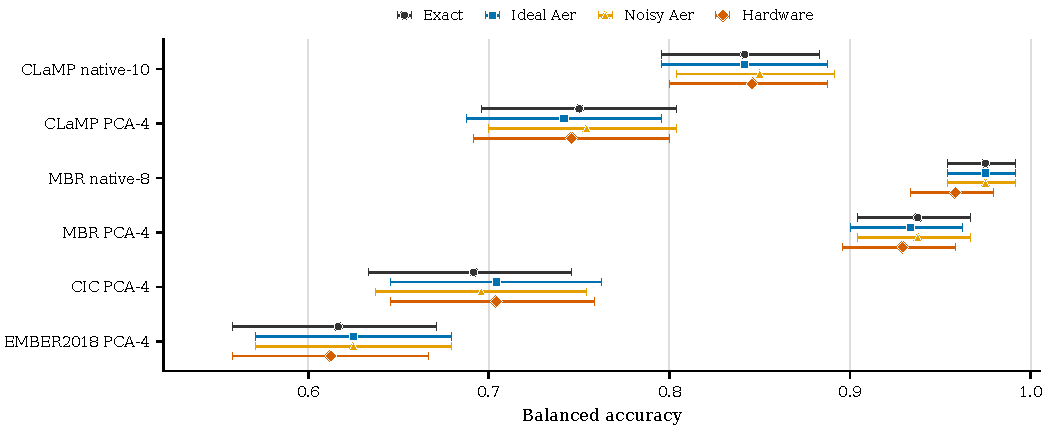
\includegraphics[width=\textwidth]{hardware_results/results/analysis/paper_figure1_execution_performance.pdf}
  \caption{Balanced accuracy across exact, ideal-Aer, noisy-Aer, and IBM hardware execution. Points are means across three held-out splits; bars are 95\% class-stratified bootstrap intervals based on 10,000 replicates and 240 held-out predictions per configuration and environment.}
  \label{fig:execution-performance}
\end{figure*}

Kernel distortion increased with circuit width (Figure~\ref{fig:kernel-distortion}). Mean hardware relative error was 0.111--0.114 for four-qubit configurations, 0.441 at eight qubits, and 0.479 at ten qubits, while hardware kernel correlations with the exact kernels remained between 0.924 and 0.997. Across the 18 primary hardware runs, CZ count correlated with relative kernel error ($r=0.857$, Spearman $\rho=0.812$) but not with hardware-minus-exact balanced accuracy ($r=-0.032$, $\rho=-0.129$).

\begin{figure*}[t]
  \centering
  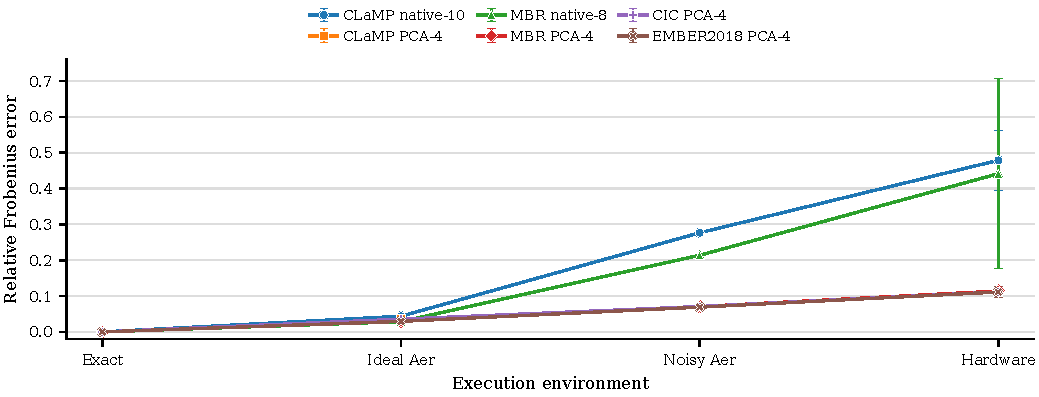
\includegraphics[width=\textwidth]{hardware_results/results/analysis/paper_figure2_kernel_distortion.pdf}
  \caption{Test-kernel relative Frobenius error against the exact statevector kernel. Markers are three-split means and error bars are split standard deviations. Exact kernels define the zero-error reference.}
  \label{fig:kernel-distortion}
\end{figure*}

PCA reduced circuit cost but produced a dataset-dependent predictive tradeoff. For CLaMP, reducing the circuit from 10 to 4 qubits lowered depth from 206 to 98 and CZ count from 70 to 22, while hardware balanced accuracy decreased by 10.0 points relative to the native representation ($p=0.0179$ after Holm adjustment). The corresponding MBR decrease was 2.9 points ($p=0.458$). The matched classical comparison in Figure~\ref{fig:quantum-classical} showed no consistent quantum advantage: RBF SVC matched or exceeded hardware-quantum performance on CLaMP, CIC, and EMBER2018, whereas the quantum kernels were descriptively higher on MBR.

\begin{figure*}[t]
  \centering
  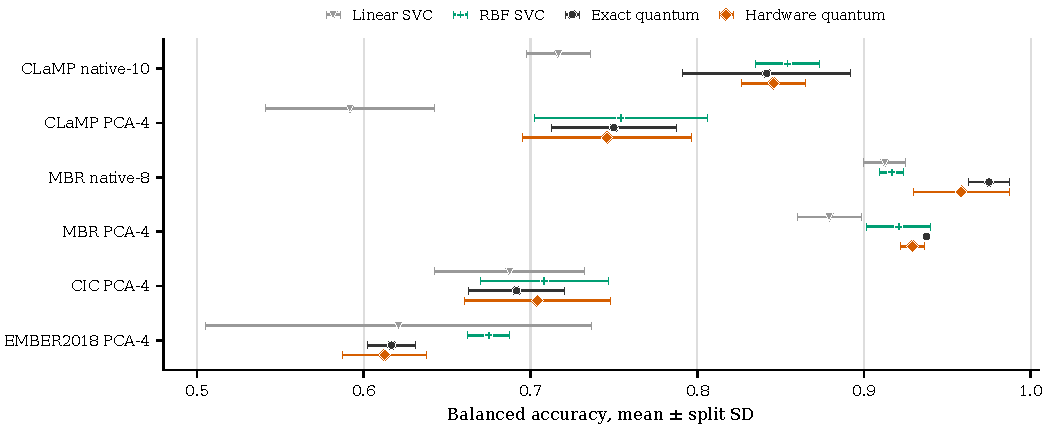
\includegraphics[width=\textwidth]{hardware_results/results/analysis/paper_figure3_quantum_classical.pdf}
  \caption{Matched linear-SVC, RBF-SVC, exact-quantum, and hardware-quantum balanced accuracy. Points are three-split means and bars are split standard deviations. Every classifier used $C=1$ without hyperparameter tuning.}
  \label{fig:quantum-classical}
\end{figure*}

The 21 hardware conditions required 102,789,120 shots and 28,189 seconds of IBM-reported QPU usage. Linear extrapolation estimated 58.3--59.0 QPU hours for 1,000 training and 1,000 test observations; this value was projected rather than directly measured.

\section{Discussion}

The principal hardware result was the stability of downstream classification despite measurable changes in the quantum kernels. Hardware execution produced substantially greater relative kernel error than exact or ideal simulation, particularly for the eight- and ten-qubit circuits, yet balanced accuracy changed by at most 1.67 percentage points in absolute value. The paired tests found no significant hardware-versus-exact prediction differences after multiplicity adjustment. These findings support empirical robustness for the tested samples, feature map, shot count, backend, and calibration period. They do not establish formal equivalence between exact and hardware execution.

Kernel fidelity and classification performance were not interchangeable measures in this experiment. CZ count was strongly associated with kernel distortion but was not associated with accuracy degradation. The hardware kernels could therefore differ numerically from their exact counterparts while retaining enough relative structure for the SVC to produce similar decision boundaries. This observation is specific to the tested SVC solutions; greater distortion could affect another dataset, feature map, regularization value, or set of support vectors differently.

Feature compression presented a separate tradeoff. Four-component PCA reduced qubit count, circuit depth, CZ count, and hardware-induced kernel distortion. It also removed predictive information in some configurations. The effect was largest for CLaMP, where PCA-4 reduced hardware balanced accuracy by 10.0 points relative to native-10. MBR showed a smaller 2.9-point reduction. The results therefore do not support treating PCA solely as a noise-reduction step: its resource benefit must be evaluated against representation loss for each dataset.

The classical comparisons did not demonstrate a consistent accuracy advantage for the quantum kernel. RBF SVC was competitive with or better than the hardware-quantum model on CLaMP, CIC, and EMBER2018, while the quantum models were descriptively higher on MBR. These comparisons used fixed $C=1$ models without hyperparameter tuning and were intended as matched checks rather than optimized classical benchmarks. The study also did not collect comparable end-to-end wall-clock or system-level energy measurements. Accordingly, the results demonstrate neither predictive, computational, nor energy-based quantum advantage.

The study has several limitations. Each split contained only 80 training and 80 test observations, and the balanced class distribution does not reflect operational malware prevalence. Only three repeated holdouts, one ZZ feature map, two repetitions, linear entanglement, 512 shots, one transpilation, and one hardware backend were evaluated. Error mitigation was disabled, and circuit width was coupled to dataset and representation, making the circuit-cost correlations descriptive rather than causal. The datasets also differ in observation type: CLaMP, MBR, and EMBER2018 describe PE files, whereas CIC represents sandbox activity records; MBR additionally depends on the provenance and version of its Kaggle source file. Finally, a post hoc CIC audit found two binary hashes recurring across different held-out splits, although no hash occurred in both training and test data within an individual split. Future work should use hash-, family-, session-, or time-grouped evaluation and repeat the experiment across devices, calibrations, feature maps, shot counts, and mitigation settings.

\section{Conclusion}

This study compared classical SVCs with exact, ideal-Aer, noisy-Aer, and IBM-hardware quantum kernels across four malware datasets. IBM hardware increasingly distorted the measured kernels as circuit width and CZ count increased, but downstream balanced accuracy remained close to exact-kernel performance in all six configurations. PCA reduced circuit cost and hardware kernel distortion while causing dataset-dependent losses in predictive performance. Classical RBF models remained competitive, and the experiment did not demonstrate quantum advantage in accuracy, speed, or energy use. The results instead provide a reproducible small-sample demonstration that quantum-kernel malware classification can remain stable on current NISQ hardware despite substantial kernel distortion.



\section{Acknowledgments}
We would like to thank the Monmouth University School of Science Summer Research Program for providing funding for this project. We would also like to thank RPI, whose on-campus IBM Quantum System One this research was conducted on.

\bibliography{aaai24}

\end{document}
